\documentclass[11pt,a4paper]{article}

\usepackage[utf8]{inputenc}
\usepackage[T1]{fontenc}
\usepackage[margin=1in]{geometry}
\usepackage{booktabs}
\usepackage{graphicx}
\usepackage{amsmath}
\usepackage[expansion=false]{microtype}
\usepackage[numbers,sort&compress]{natbib}
\usepackage[colorlinks=true,allcolors=blue]{hyperref}

% Arm names, so a rename is one edit.
\newcommand{\armbzs}{\texttt{BZS}}
\newcommand{\armbzz}{\texttt{BZZ}}
\newcommand{\armbzzu}{\texttt{BZZU}}
\newcommand{\armbzsz}{\texttt{BZSZ}}
\newcommand{\armbzp}{\texttt{BZP}}

% Generated from RESULTS/boltz/*/metrics.json by paper/make_tables.py.
% Generated by paper/make_tables.py -- do not edit by hand.
\newcommand{\ntest}{8450}
\newcommand{\ntrain}{17744}
\newcommand{\nval}{1972}
\newcommand{\ntotal}{28166}
\newcommand{\nsplits}{5}
\newcommand{\targetfixes}{26}
\newcommand{\bzzupca}{0.821}
\newcommand{\bzzupcasd}{0.017}
\newcommand{\bzzupcadelta}{+0.0543}
\newcommand{\onehotrho}{0.767}
\newcommand{\onehotsd}{0.018}
\newcommand{\onehotunseen}{1.643}
\newcommand{\bzzuunseen}{1.365}
\newcommand{\bzsrho}{0.747}
\newcommand{\bzzrho}{0.748}
\newcommand{\bzpflat}{0.260}
\newcommand{\bzzuvariance}{78.4}
\newcommand{\bzsvariance}{40.4}
\newcommand{\bzzuflat}{0.836}
\newcommand{\bzzuflatdelta}{+0.0694}


\title{Structure-conditioned representations predict peptide--HLA
complex lifetime where protein language models do not}

\author{Noe Obersteiner \and Lorenzo Mensi}
\date{\today}

\begin{document}
\maketitle

\begin{abstract}
\noindent
The kinetic stability of a peptide--HLA class~I complex predicts T~cell
immunogenicity better than binding affinity does, which makes complex
half-life the quantity worth modelling for epitope and vaccine design. We
report a controlled comparison of input representations for this target on
\ntotal{} measured nine-mer--HLA pairs across 75 alleles. A one-hot encoding of
the 43 peptide and groove-contact positions is a strong baseline, and frozen
ESM-2 embeddings of those same positions do not beat it at any layer. Frozen
embeddings from Boltz-2, a structure-prediction model, do: contracting its
\emph{pair} representation over the peptide--groove interface reaches Spearman
$\rho = \bzzupca{} \pm \bzzupcasd{}$ against the baseline's $\onehotrho{} \pm
\onehotsd{}$, winning all \nsplits{} splits at an identical 860-feature budget,
and reduces error on held-out alleles by 17\%. The arm built on Boltz-2's
\emph{single} representation reproduces the language-model result instead. We
argue the asymmetry is not about information---the pair tensor is a
deterministic function of the two sequences---but about which computation is
already done. Complex lifetime is set by an escape barrier that depends on
residue--residue complementarity, and a pairwise representation supplies that
functional form directly, where a per-residue sequence model leaves it to be
learned from labels. We state the controls this result still needs.
\end{abstract}

\section{Why complex lifetime}
\label{sec:why}

A peptide presented on an HLA class~I molecule is only visible to a T~cell for
as long as the complex survives at the cell surface. \citet{rasmussen2016}
measured the dissociation half-life of \ntotal{} nine-mer--HLA complexes across
75 alleles and showed that this stability is a \emph{better} correlate of
immunogenicity than binding affinity---the quantity most presentation
predictors are trained on. For epitope selection and vaccine design, the
practical question is therefore not only whether a peptide binds but how long
the complex lasts.

That shift in target has a modelling consequence that is easy to overlook.
Affinity is a thermodynamic quantity, a free-energy difference between bound
and unbound states. Half-life is \emph{kinetic}: it is governed by
$k_{\mathrm{off}}$, hence by the height of the barrier to peptide escape from
the groove. A barrier is a property of the assembled complex along a
dissociation path---how deeply the P2 and P9 anchor side chains are buried in
the B and F pockets, which hydrogen bonds to the conserved groove residues must
break, and how those contributions couple. It is not a sum of independent
per-residue preferences.

\section{Dataset and evaluation}
\label{sec:data}

We use the \citet{rasmussen2016} dataset: \ntotal{} peptide--HLA pairs with
measured half-life in hours, 75 HLA molecules, all peptides nine residues. The
regression target is $\ln(t_{1/2} + 0.1)$; the offset keeps the 20\% of rows
measured at the assay's zero floor only $0.22$ standard deviations from the
next observed value rather than at $-\infty$.

Each HLA molecule is represented by the 34 groove positions that
\citet{reynisson2020} identify as peptide-contacting---residues within
4.0\,\AA{} of the bound peptide in pMHC crystal structures---giving, with the
nine peptide positions, 43 \emph{slots} per complex. Every representation in
this paper describes those same 43 slots, so the comparison isolates how a
position is encoded, not which positions are seen.

We evaluate on \nsplits{} moment-matched splits
(\ntrain{}/\nval{}/\ntest{} rows train/validation/test). Within each split the
test set contains rows whose peptide is unseen in training and rows whose
\emph{allele} is unseen in training; we report error on the unseen-allele
stratum separately, because generalising to an allele with no labels is the
regime that matters for a pan-specific predictor and the regime where
memorisation cannot help.

Every representation is scored through an identical regression head---an MLP
with hidden widths $256$ and $128$, dropout $0.2$, Adam, MSE on the
standardised target, early stopping on a 10\% slice carved out of training.
All fitted transforms (any projection, the feature standardiser, the target
centering) are fitted on training rows only; the early-stopping slice is
excluded from each of them and the test set is scored once. Split $i$ uses
seed $i$ for every representation, so comparisons are paired.

\section{Protein language model embeddings do not beat one-hot}
\label{sec:plm}

A one-hot encoding of 43 positions over the 20-letter amino acid alphabet is
860 features and, for per-residue information, is complete: it is an exact,
lossless description of what residue sits at each slot. Our baseline reaches
$\rho = \onehotrho{} \pm \onehotsd{}$.

Frozen ESM-2 \citep{lin2023} embeddings of the same 43 positions do not improve
on it. Across layers 0, 15 and 33 of the 650M-parameter model, no arm beats the
baseline by more than its split-to-split spread, and the deepest layers are
slightly worse. Layer~0 provides a useful null: ESM-2's input embedding has rank
20 on a 20-letter alphabet, so it is an invertible linear reparameterisation of
one-hot and carries exactly the same information. It ties with the baseline,
which is what a correct pipeline must produce, and confirms the comparison is
measuring representation rather than plumbing.

\section{Why that was the expected outcome}
\label{sec:expected}

A protein language model returns, for each residue, a vector summarising that
residue's context under the evolutionary statistics of single sequences. Two
properties of our setup make that nearly useless here.

First, the positions are fixed and few. We do not need a model to tell us
\emph{which} residues matter; \citet{reynisson2020}'s contact analysis already
fixed the 43 slots. What remains is to encode the identity at each slot, and
one-hot does that exactly. A frozen per-residue embedding can only
re-parameterise information the baseline already has in full, and any
compression of it can only lose.

Second, the context a language model supplies is the wrong context. ESM-2
embeds the HLA as a protein among proteins; it has no representation of
\emph{this} peptide sitting in \emph{this} groove, because it never sees the two
chains together. The quantity we want depends on exactly that joint object.

\section{Why a structure model is the right instrument}
\label{sec:boltz}

Boltz-2 \citep{boltz2} predicts biomolecular complex structure, and internally
maintains two trunk representations: a \emph{single} representation $s$, one
vector per token, and a \emph{pair} representation $z$, one vector per
\emph{ordered pair} of tokens, refined over the actual two-chain complex.

The pair representation is the interesting one, and the reason is the physics of
Section~\ref{sec:why}. An escape barrier is built out of residue--residue
contacts and the couplings between them. A representation indexed by residue
pairs and conditioned on both chains jointly has that functional form already;
a per-residue representation does not, and a regression head on top of one must
construct pairwise interactions itself, from labels.

It is worth being precise about what is and is not being claimed. Boltz-2 adds
no \emph{information}: $z = f(\text{peptide}, \text{HLA})$ is a deterministic
function of the two sequences, which the one-hot input already determines. In
the Shannon sense there is nothing in $z$ that is not in the baseline's input.
The claim is about \emph{amortised computation and inductive bias}. Our head is
a two-layer MLP with \ntrain{} training rows spread over 75 alleles; learning a
useful pairwise interaction map from that is a hard estimation problem. Boltz-2
performed an equivalent computation during its own pretraining, supervised by
structure---a signal orthogonal to our labels and vastly more abundant. Using
$z$ is a way of importing that computation rather than repeating it.

This predicts something specific and falsifiable: the advantage should be
largest on \emph{unseen alleles}. A one-hot model must learn allele-specific
weights and has nothing to apply to an allele it never saw, whereas a pairwise
interaction map is about complementarity and should transfer.

\paragraph{Why not Boltz-2's own affinity head.}
Boltz-2 ships a binding-affinity module, which would be the obvious first
thing to try, and it cannot be used here. Its PairFormer attends only over
protein--ligand and intra-ligand interactions, so the peptide--protein
interface is outside what it models; the interface requires the binder as a
ligand chain capped at 128 atoms; and affinity training discarded ligands above
50 heavy atoms, while these nine-mers carry 48--100 (median 75). The route is
closed at the interface, the atom cap and the training distribution
independently. We therefore build a head on the frozen trunk, as
\citet{prefolddg} do for protein--protein $\Delta G$.

\section{Method}
\label{sec:method}

Boltz-2 is run once per complex and is \textbf{frozen throughout}; nothing in it
is trained. For each complex we keep the trunk's $s$ ($[191, 384]$) and $z$
($[191, 191, 128]$), where $191 = 182$ HLA residues $+$ 9 peptide residues, and
reduce each to the 43 slots of Section~\ref{sec:data}. This yields four
representations:

\begin{itemize}
  \item \armbzs{}: $s$ gathered at the 43 slots. The single-representation
        control, and the direct analogue of the ESM-2 arms.
  \item \armbzz{}: $z$ contracted over the peptide--groove interface with
        inverse-square distance weights, following \citet{prefolddg}.
  \item \armbzzu{}: the same contraction with uniform weights.
  \item \armbzp{}: the confidence module's per-token pLDDT at the 43 slots.
\end{itemize}

For peptide slot $p$ and contact position $q$, writing
$z^{\mathrm{blk}}_{pq} = \tfrac{1}{2}(z_{p q} + z_{q p})$ to symmetrise, the
contraction is
\begin{equation}
  \tilde z_p = \frac{\sum_q w_{pq}\, z^{\mathrm{blk}}_{pq}}{\sum_q w_{pq}},
  \qquad
  \tilde z_{9+q} = \frac{\sum_p w_{pq}\, z^{\mathrm{blk}}_{pq}}{\sum_p w_{pq}},
\end{equation}
with $w_{pq} = 1/\max(d_{pq}, 3.0)^2$ for \armbzz{} and $w_{pq} = 1$ for
\armbzzu{}; $d_{pq}$ is the C$\alpha$--C$\alpha$ distance in the predicted
structure. Both contraction directions are kept, so the result retains
per-position structure: collapsing the peptide axis would destroy the anchor
identity that dominates class~I binding, which is why we diverge from
\citet{prefolddg}'s outer-product pooling (that pooling exists to give
variable-length complexes a fixed-size vector; ours are always $182 + 9$).

Slots are then pooled to a fixed width. \texttt{pca:20} projects each slot to 20
principal components fitted on training rows, giving every arm exactly 860
features and a byte-identical head---this is the budget-matched setting and the
one we treat as load-bearing. \texttt{flatten} keeps all $43 \times D$ features
and is therefore \emph{not} budget-matched; we report it to bound what the
compression costs, not as evidence about representations.

\paragraph{Conditions.} Two deliberate cost choices should be read alongside
every number below. Extraction ran with \texttt{sampling\_steps}~$=10$ against
Boltz-2's default of 200, and with \emph{no multiple sequence alignment} on
either chain. Boltz-2 itself warns that single-sequence mode degrades
predictions, so the structural inputs here are of knowingly reduced fidelity.

\section{Results}
\label{sec:results}

\begin{table}[t]
\centering
\small
\begin{tabular}{llrrrr}
\toprule
Representation & Feat. & Spearman $\rho$ & RMSE & Unseen-HLA & $\Delta\rho$ (won) \\
\midrule
A0 one-hot & 860 & $0.767 \pm 0.018$ & 1.172 & 1.643 & reference \\
\armbzs{} single $s$ & 860 & $0.747 \pm 0.023$ & 1.203 & 1.583 & -0.0194 (0/5) \\
\armbzz{} pair, $1/d^2$ & 860 & $0.748 \pm 0.012$ & 1.207 & 1.450 & -0.0191 (0/5) \\
\armbzsz{} single $+$ pair & 860 & $0.765 \pm 0.014$ & 1.165 & 1.451 & -0.0017 (3/5) \\
\bfseries \armbzzu{} pair, uniform & 860 & $0.821 \pm 0.017$ & 1.036 & 1.365 & +0.0543 (5/5) \\
\bottomrule
\end{tabular}
\caption{Budget-matched comparison (\texttt{pca:20}). Every arm is compressed to 860 features, so the regression head is byte-identical across rows and only the input representation differs. RMSE is in log units; Unseen-HLA is RMSE restricted to test rows whose allele does not appear in training. $\Delta\rho$ is paired split by split against A0.}
\label{tab:pca20}
\vspace{2pt}\footnotesize Mean $\pm$ SD over \nsplits{} splits, one seed per split; the SD is split spread, not seed spread (\S\ref{sec:limits}).
\end{table}

\begin{table}[t]
\centering
\small
\begin{tabular}{llrrrr}
\toprule
Representation & Feat. & Spearman $\rho$ & RMSE & Unseen-HLA & $\Delta\rho$ (won) \\
\midrule
A0 one-hot & 860 & $0.767 \pm 0.018$ & 1.172 & 1.643 & reference \\
\armbzs{} single $s$ & 16512 & $0.786 \pm 0.021$ & 1.120 & 1.507 & +0.0188 (5/5) \\
\armbzz{} pair, $1/d^2$ & 5504 & $0.782 \pm 0.013$ & 1.132 & 1.379 & +0.0157 (4/5) \\
\armbzsz{} single $+$ pair & 22016 & $0.805 \pm 0.013$ & 1.072 & 1.395 & +0.0378 (5/5) \\
\bfseries \armbzzu{} pair, uniform & 5504 & $0.836 \pm 0.015$ & 0.992 & 1.292 & +0.0694 (5/5) \\
\bottomrule
\end{tabular}
\caption{Uncompressed comparison (\texttt{flatten}). This row set is \emph{not} budget-matched: the Boltz arms carry more features, and hence more first-layer parameters, than A0. It bounds what the compression in Table~\ref{tab:pca20} costs, and is not evidence about representation quality on its own.}
\label{tab:flatten}
\vspace{2pt}\footnotesize Mean $\pm$ SD over \nsplits{} splits, one seed per split.
\end{table}


\begin{figure}[t]
\centering
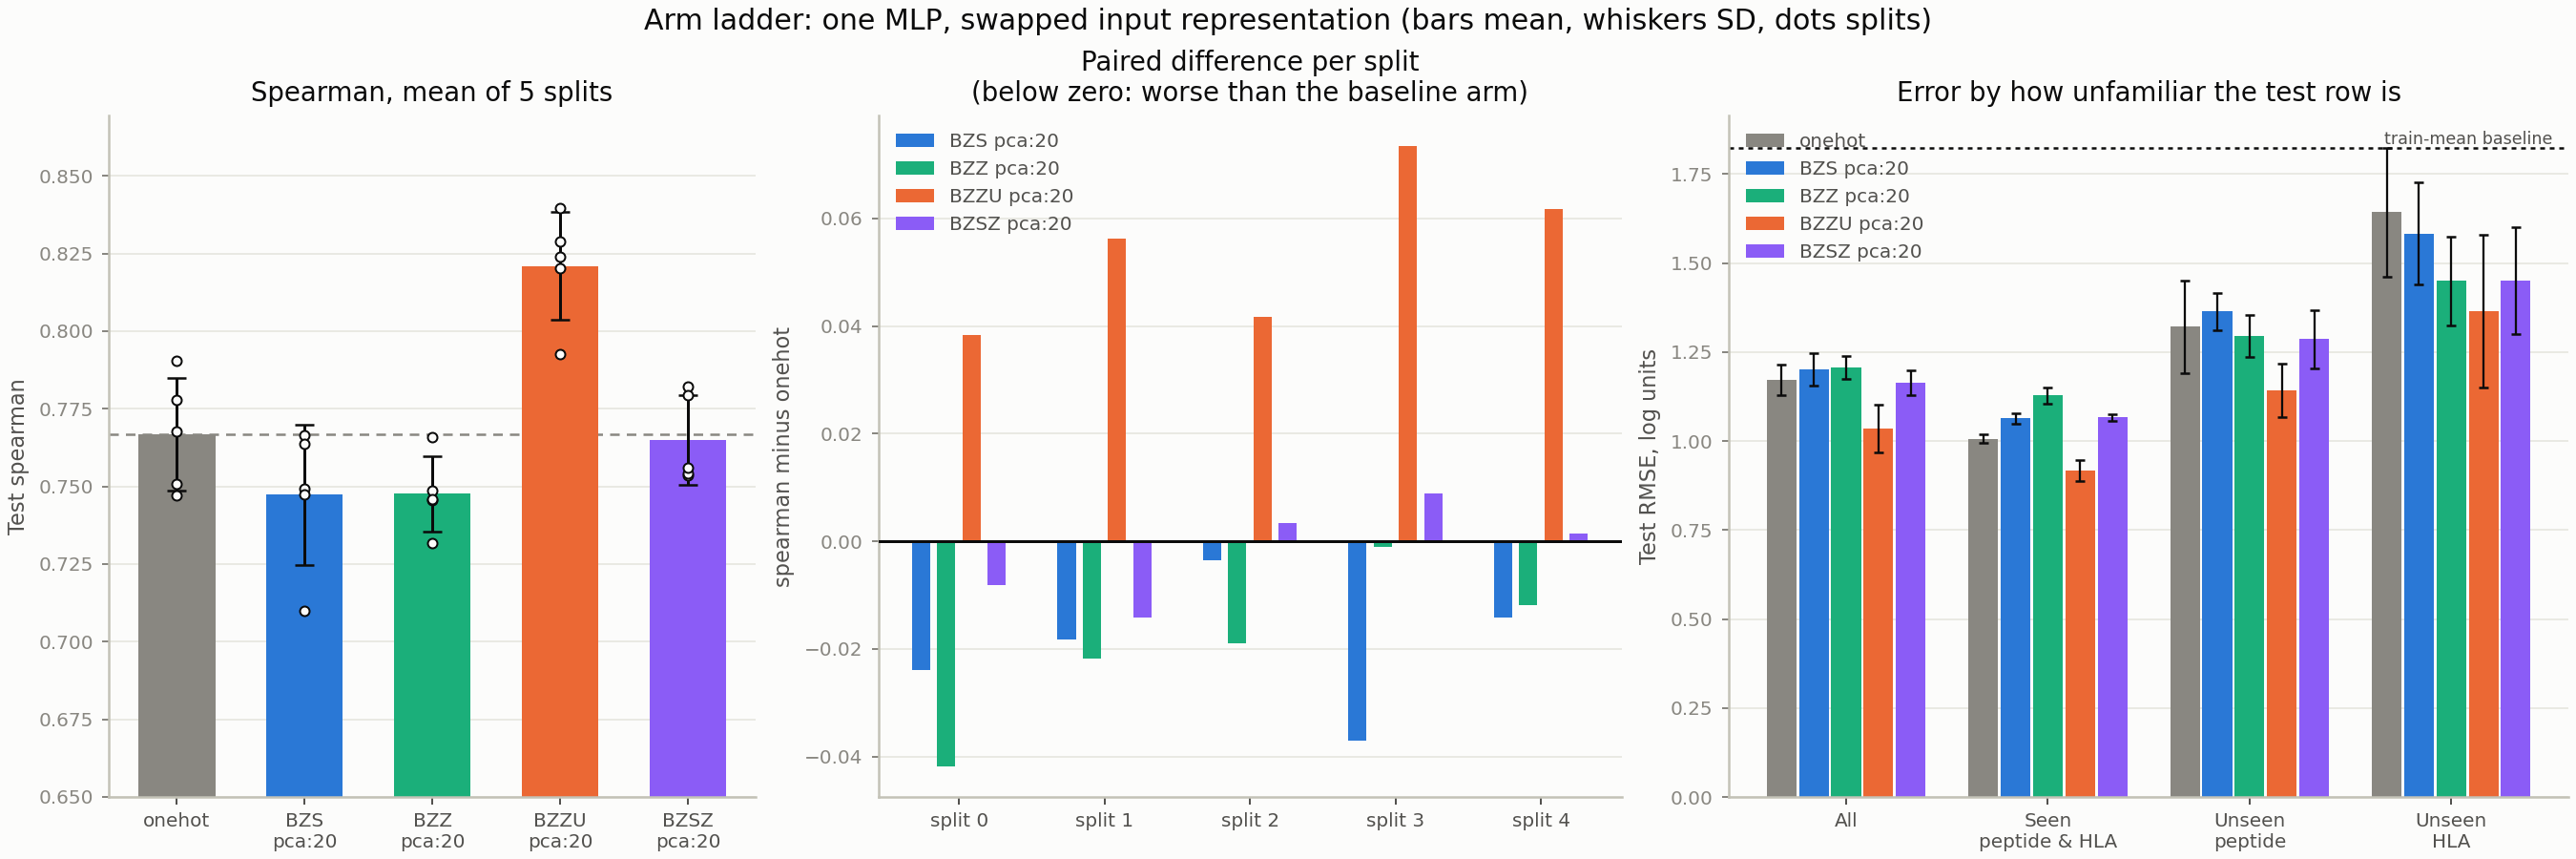
\includegraphics[width=\linewidth]{figures/ladder_boltz_pca20.png}
\caption{The budget-matched ladder (\texttt{pca:20}), all arms at 860 features
through an identical head. Only \armbzzu{}, the uniform interface contraction
of Boltz-2's pair representation, clears the one-hot baseline; the
single-representation arm \armbzs{} falls below it, as the frozen ESM-2 arms do.
Error bars are spread across the \nsplits{} splits, which is shared between arms
(\S\ref{sec:limits}).}
\label{fig:ladder}
\end{figure}

Table~\ref{tab:pca20} is the comparison we consider decisive. At an identical
860-feature budget, \armbzzu{} reaches $\rho = \bzzupca{} \pm \bzzupcasd{}$
against the baseline's $\onehotrho{}$, a paired gain of \bzzupcadelta{} that
holds on all \nsplits{} splits. No ESM-2 arm achieves this at any layer or
pooling.

Three further readings matter more than the headline.

\paragraph{The pair tensor is what carries it.} \armbzs{}, built on Boltz-2's
single representation, reaches only $\bzsrho{}$---below the one-hot baseline,
reproducing the language-model result of Section~\ref{sec:plm} with a different
model. The gain is not "a bigger foundation model"; Boltz-2's single
representation is 384-dimensional against ESM-2 650M's 1280 and is not the
richer per-residue featurizer. What distinguishes \armbzzu{} is that it is
indexed by residue pairs and conditioned on the complex.

\paragraph{The gain is largest where transfer is required.} On test rows whose
allele never appears in training, RMSE falls from $\onehotunseen{}$ to
$\bzzuunseen{}$, a 17\% reduction, and the same ordering holds under
\texttt{flatten} (Table~\ref{tab:flatten}). This is the prediction of
Section~\ref{sec:boltz} landing: a pairwise complementarity map transfers to an
unlabelled allele in a way that allele-specific one-hot weights cannot. We
regard this, not the aggregate $\rho$, as the strongest evidence that something
structural is being used.

\paragraph{Confidence alone is weak.} \armbzp{}, which trains on nothing but 43
pLDDT scalars already computed on every run, reaches $\bzpflat{}$. That is far
above chance from a representation that costs nothing extra, and far below any
sequence representation. We draw no conclusion from it: without a sequence-only
control matched on peptide composition we cannot say whether it reflects
complex stability or merely which peptides are easy to place.

\subsection{Uniform versus distance-weighted contraction}

\armbzzu{} (uniform) outperforms \armbzz{} (inverse-square) by a wide margin,
$\bzzupca{}$ against $\bzzrho{}$. Taken at face value this is backwards: the arm
that discards the predicted geometry wins.

We think the most likely explanation is the extraction conditions above, not a
claim about distance weighting in principle. \armbzzu{} reads only the
Pairformer's learned pair representation, which is refined by triangle attention
and already reflects pairwise proximity. \armbzz{} multiplies into that a
geometric weight computed from a single diffusion sample drawn at 10 sampling
steps without any MSA---so where the coordinates are unreliable, the weighting
injects per-row noise and sharply discounts contacts beyond about 5\,\AA{} on
that unreliable basis. Consistent with noise rather than breakage, \armbzz{}
still achieves the second-best unseen-allele RMSE in Table~\ref{tab:flatten}
($1.379$); a corrupted feature would not.

This remains a hypothesis. We have audited the contraction code and found the
two arms share a single implementation differing only in the weight array, with
consistent index spaces and no degeneracy in the distance floor, so the gap is
not an indexing bug. Discriminating noise from principle requires re-extracting
a sample at default sampling steps with real alignments, which we have not done.

\section{Limitations and outstanding controls}
\label{sec:limits}

We would rather state these than have them found.

\begin{enumerate}
  \item \textbf{One seed per split.} Each arm was run once per split, with
        seed $=$ split index. The $\pm$ figures throughout are therefore
        \emph{split} spread, which is shared across arms and dominated by split
        difficulty; they are not seed spread, and we have no estimate of
        seed-to-seed variance. Our own experience on this pipeline is that
        pooling and standardisation choices alone move $\rho$ by about $0.025$
        on identical information, which is within a factor of about two of the
        reported effect. Replicate seeds are the single most important
        outstanding run.
  \item \textbf{The baseline and the arms differ by more than representation.}
        Under the default policy the one-hot baseline is left unstandardised,
        while every Boltz arm passes through a fitted per-dimension prescaling
        and a fitted feature standardiser with clipping. One-hot is already
        unit-scale, which is the rationale, but it means the budget-matched
        comparison is not a pure representation swap. We ran the control:
        putting the baseline through the standardiser moves it from
        $0.7687 \pm 0.0217$ to $0.7742 \pm 0.0161$, a paired gain of
        $+0.0055$ winning 3 of \nsplits{} splits. The asymmetry is therefore
        worth roughly a tenth of the \bzzupcadelta{} it was feared to explain,
        and the headline survives it. Two caveats: this control ran against the
        uncorrected target, so it is a within-baseline paired comparison rather
        than a drop-in replacement for the reference row; and its
        \texttt{never} arm reproduces the committed baseline to $0.002$, which
        is itself a useful bound on environment-to-environment drift.
  \item \textbf{\texttt{flatten} is a capacity comparison.} In
        Table~\ref{tab:flatten} the Boltz arms carry up to 22{,}016 features
        against the baseline's 860, and correspondingly more first-layer
        parameters. The \texttt{flatten} gain should not be read as a
        representation result. Relatedly, the one-hot arm ignores the pooling
        flag---it is the same 860-feature configuration in every row---so its
        value is repeated rather than re-measured across pooling settings.
  \item \textbf{\texttt{pca:20} is not neutral between arms.} Projecting to 20
        components per slot retains \bzzuvariance{}\% of \armbzzu{}'s variance
        but only \bzsvariance{}\% of \armbzs{}'s, and would retain a far smaller
        fraction of a 1280-dimensional ESM-2 arm's. The setting equalises
        feature count, not information, and it is more forgiving to
        low-dimensional representations. It is fair against one-hot, which is
        uncompressed at 860 features; it is \emph{not} a fair
        Boltz-versus-ESM-2 comparison, and we do not use it as one.
  \item \textbf{Degraded structural inputs.} 10 sampling steps and no MSA, as
        described in Section~\ref{sec:method}. We read this as evidence the
        result is robust---it was obtained with a deliberately weakened
        Boltz-2---but the measurement of what those choices cost has not been
        made.
  \item \textbf{A missing null.} We have not run a random-projection arm at 860
        features, nor an arm from a randomly initialised Boltz-2. Either would
        test directly whether the gain comes from the trained representation
        rather than from dimensionality or pipeline details.
  \item \textbf{Target provenance.} The half-life column in the distributed
        spreadsheet was partly mangled into datetimes, and the inversion is not
        lossless: values of the form $x.0Y$ collapse, so a true $1.05$ recovers
        as $1.5$. All arms here are trained against a corrected target
        (\targetfixes{} rows differ), applied identically, so the comparison is
        unaffected---but the corrected file is not currently committed
        alongside the code, and should be.
\end{enumerate}

None of these is reason to discount the central observation: at a matched
budget, on identical rows, with a paired design and a clean train/test
discipline, a structure-conditioned pair representation beats a complete
per-residue encoding on this target, and does so by the largest margin exactly
where generalisation to new alleles is required. They are reasons to run three
more experiments before the margin is quoted as a number rather than as a
direction.

\bibliographystyle{plainnat}
\bibliography{refs}

\end{document}
